\section{System Framework}
In this section, we present the system diagram (Figure
\ref{fig:framework}), which shows how data flows through our system
end-to-end.  Just like classical IR systems, it can be divided into
online and offline components.

\begin{figure}[!htbp]
\centering
%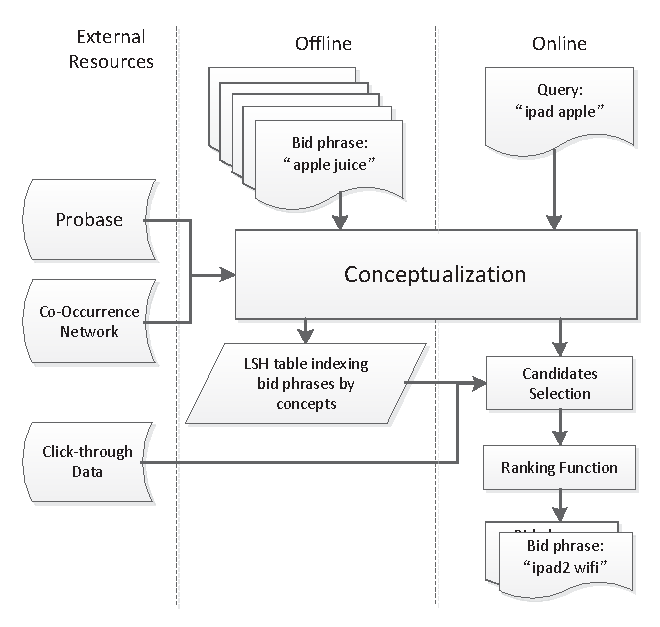
\epsfig{file=figures/frameworkv2.eps, width=3.3in}
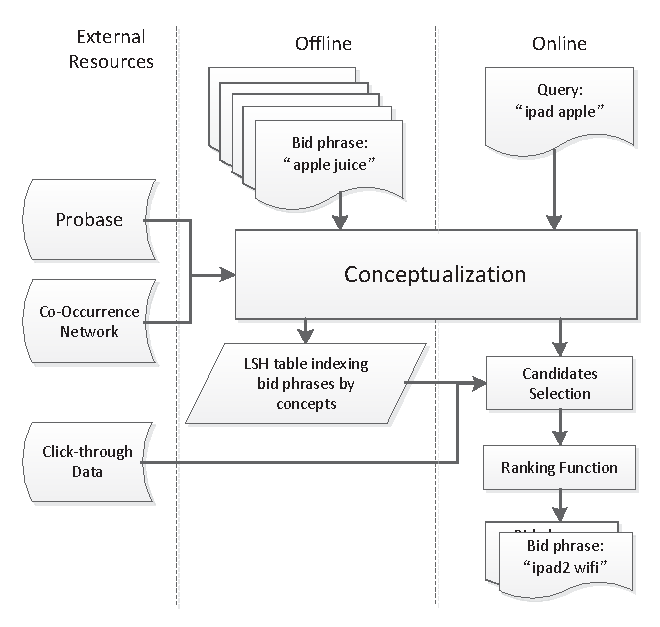
\includegraphics[width=3.3in]{figures/frameworkv2.eps}
\caption{Overall System Architecture}
\label{fig:framework}
\end{figure}
%We also include a module in our framework that evaluate and tune the
%resulting suggestions(expansions) based on statistics collected from
%actual combat.



In offline processing, we conceptualize each bid phrase, that is, we
map each bid phrase to a set of representative concepts.  This enables
us to estimate the similarity between two short texts by measuring the
similarity between their corresponding sets of concepts.  For the
purpose of large scale similarity computation, we exploit the
locality-sensitive hash (LSH) scheme to index bid phrases.  LSH
enables us to efficiently find bid phrases whose corresponding concept
sets are likely to be similar to that of the query.  Besides, we also
mine click-through data to extract semantic associations (i.e.,
co-click relationships) between queries and index them for efficient
real-time looking up.  At runtime, when a query is posed, we
conceptualize it in the same way as we did for bid phrases.
%Because the number of bid phrases contained by search engine is
%extremely large, comparing a given query with each bid phrase on
%their rich conceptualization results can't satisfy efficiency
%requirements of online system.
%Because the number of bid phrases is usually in the order of
%billions, it is not feasible to compare the concept representation of
%the query with that of each bid phrase.  In order to make our approach
%efficient enough to handle the massive amount of bid phases, we
Then, from the massive bid phrase dataset, we select a small
set of bid phrases that are relevant to the given query using 
user behavior data (for head queries) or 
%and 
LSH (for tail queries).
%portion from the entire corpus of
%bid phrases as candidates that are somewhat relevant to the given query.%for further consideration.
Finally, we rank these candidates and use the top-ranking ones as
query suggestions (expansions).
%If the given query has enough
%For queries that have sufficient click-trhough data to draw reliable
%conclusion on which bid phrases are relevant to it, we select bid
%phrases as candidates for it based on such information.
% If the query is a term of our pre-built index that contains co-click
% relationships, we simply select bid phrases from the posting list of
% the term as candidates.
% Otherwise, we look the conceptualization result
% of the given query up in the LSH tables and use retrieved bid phrases as
% candidates.
%Finally, we apply our ranking function to re-order
%selected candidates and reserve the top ranking ones as final results.



%Such task should be finished efficiently while ensuring the quality of
%candidates.
%We design two approaches for candidates selection.
%One approach leverage semantic associations provided by click-through
%data by looking up our lookup table to select associated search phrases.
%So our another approach only focus on conceptualization results.
%we look the conceptualization result of given query up in
%the LSH table and use those retrieved bid phrases as candidates.
%As an efficient real-time system, we can apply our approach to
%preprocess a large collection of queries without any additional
%difficulty.
%The resulting lists of bid keywords can be used as suggested keywords
%or query's expansions for sponsored search.
%Actually, we use a small portion of search engine's traffic volume to
%evaluate our results.
%According to collected statistics, we tune the setting of our approach
%improve better suggestions(expansions).
%\comment{{do we need to claim we get good resutls in the flight?}}


%%% Local Variables:
%%% mode: latex
%%% TeX-master: "adselection"
%%% End:
